\documentclass[14pt]{article}
\usepackage[cp1251]{inputenc}
\usepackage[T2A]{fontenc}
\usepackage[russian]{babel}
\usepackage{indentfirst}
\usepackage{amsmath}
\usepackage{amsfonts}
\usepackage{floatrow}
\usepackage{graphicx}
\usepackage{vmargin}
\setpapersize{A4}
\setmarginsrb{2.5cm}{2cm}{2cm}{3cm}{0pt}{0mm}{0pt}{26mm}

\begin{document}

\begin{titlepage}

\begin{centering}
Ìèíèñòåðñòâî îáðàçîâàíèÿ è íàóêè Ðîññèéñêîé Ôåäåðàöèè\\
Ìîñêîâñêèé ãîñóäàðñòâåííûé óíèâåðñèòåò èìåíè Ì.Â.Ëîìîíîñîâà\\
Ôàêóëüòåò âû÷èñëèòåëüíîé ìàòåìàòèêè è êèáåðíåòèêè\\
Êàôåäðà îïòèìàëüíîãî óïðàâëåíèÿ\\

\vfill
\LARGE
\textbf{Îò÷¸ò ïî çàäàíèÿì ïðàêòèêóìà}\\
\textbf{Ðåøåíèå ïðèêëàäíûõ çàäà÷ îïòèìàëüíîãî óïðàâëåíèÿ â ïàêåòå GAMS}\\

\vfill

\end{centering}

\begin{flushright}

Âûïîëíèëà ñòóäåíòêà\\
5 êóðñà, 513 ãðóïïû,\\
Êîçëîâà Ìàðèÿ Ñåðãååâíà\\

\vspace{0.7cm}

Ðóêîâîäèòåëü:\\
Ãðèãîðåíêî Íèêîëàé Ëåîíòüåâè÷\\

\end{flushright}

\vfill

\centerline{Ìîñêâà}
\centerline{2013}

\end{titlepage}

\pagebreak

\setcounter{page}{2}

\tableofcontents

\newpage

\section{Îïòèìèçàöèÿ ïèòàíèÿ è èíúåêöèé èíñóëèíà ïðè ñàõàðíîì äèàáåòå}
\subsection{Ïîñòàíîâêà çàäà÷è}

Äèíàìèêà ñàõàðà è èíñóëèíà â êðîâè îïèñûâàåòñÿ ñëóäóþùèìè óðàâíåíèÿìè:

\begin{equation}\label{syst1}
\left\{ \begin{aligned}
& \frac{dy}{dt} = b_1(x-x_{0})H(x-x_{0}) - b_2 y+b_{3}\omega(t), \; y(0) = 0, \\
& \frac{dx}{dt} = - a_{1}xy+a_2(x_0-x)H(x_0-x)-a_4(x-x_0)H(x-x_0)+a_3 z(t), \; x(0) = x^0,
\end{aligned}\right.
\end{equation}
ãäå

$$
H(\xi) = \begin{cases} 1, & \xi \ge 0 \\ 0, & \xi < 0 \end{cases}.
$$

Ãðàôèê ïðèåìà ïèùè çäîðîâûì ÷åëîâåêîì:
\begin{equation}\label{z1}
z^1(t) = \begin{cases}
           50,& t \in [8, 8.3], \\
           100 , & t \in [12, 12.3], \\
           100 , & t \in [18,18.3],\\
           0, & \mbox{èíà÷å}. \\
\end{cases}
\end{equation}

Ïóñòü $ x^1(t), y^1(t) $ - ðåøåíèå ñèñòåìû ïðè ïàðàìåòðàõ çäîðîâîãî ÷åëîâåêà.

\textbf{Çàäà÷à 1}. Ïðè ïàðàìåòðàõ îðãàíèçìû áîëüíîãî äèàáåòîì ñðåäíåé òÿæåñòè è $z(t)$ âèäà \eqref{z1} íàéòè
$$
J_1 = \int_0^{24} \Big( A(x(t)-x^1(t))^2 + B\omega^2(t)\Big) dt \rightarrow \min_{\omega(t)}.
$$

\textbf{Çàäà÷à 2}. Ïðè ïàðàìåòðàõ îðãàíèçìû áîëüíîãî äèàáåòîì ñðåäíåé òÿæåñòè íàéòè
$$
J_2 = \int_0^{24} \Big( A(x(t)-x^1(t))^2 + B\omega^2(t) + C(z(t)-z^1(t))^2 \Big) dt \rightarrow \min_{z(t),\omega(t)}.
$$

\subsection{Çàäà÷à íåëèíåéíîãî ïðîãðàììèðîâàíèÿ}

Ïåðåõîäèì ê çàäà÷å íåëèíåéíîãî ïðîãðàììèðîâàíèÿ ñ ïîìîùüþ ðàçíîñòíîé ñõåìû Ýéëåðà ñ øàãîì $h=\frac{T}{n}$:

\begin{equation}\label{NLP1}
\left\{ \begin{aligned}
& \frac{y_{k+1}-y_k}{h} = b_1(x_k-x_0)H(x_k-x_0) - b_2 y_k+b_{3}\omega_k, \\
& \frac{x_{k+1}-x_k}{h} = - a_{1}x_k y_k+a_2(x_0-x_k)H(x_0-x_k)-a_4(x_k-x_0)H(x_k-x_0)+a_3 z_k,\; k = \overline{0,n-1} \\
& y_0 = 0 , x_0 = x^0.
\end{aligned}\right.
\end{equation}

Èíòåãðàëû ñ÷èòàåì ìåòîäîì ïðÿìîóãîëüíèêîâ:

$$
    J_1 =\sum_{i=0}^n A(x_k-x_k^1)^2 h + \sum_{i=1}^n B\omega_k^2 h,
$$

$$
    J_2 =\sum_{i=0}^n A(x_k-x_k^1)^2 h + \sum_{i=1}^n B\omega_k^2 h + \sum_{i=1}^n C(z_k - z_k^1)^2 h.
$$


\subsection{Ðåøåíèå â GAMS}

Çíà÷åíèå ôóíêöèîíàëà â ïåðâîé çàäà÷å ïðè ïàðàìåòðàõ: $A=1,\;B=0.01$, ïîëó÷èëîñü ðàâíûì: $J_1 = 30.7$; âî âòîðîé çàäà÷å ïðè ïàðàìåòðàõ: $A=1,\;B=0.01,\; C=0.1$, $J_2 = 30.1$.

Ãðàôèê îòêëîíåíèÿ óðîâíÿ ñàõàðà â êðîâè áîëüíîãî ÷åëîâåêà îò çäðîâîãî, à òàêæå îïòèìàëüíûé óðîâåíü èíúåêöèé ïðåäñòàâëåíû íà Ðèñ.\ref{task1_dx} è Ðèñ.\ref{task1_w} ñîîòâåòñòâåííî.
%Âî âòîðîé çàäà÷å îòêëîíåíèå ãðàôèêà îïòèìàëüíîãî ïðèåìà ïèùè äëÿ áîëüíîãî ÷åëîâåêà ïî îòíîøåíèþ ê ãðàôèêó ïðèåìà ïèùè çäîðîâîãî ÷åëîâåêà íåçíà÷èòåëüíîå.
Íà Ðèñ. \ref{task1_dz} ïîêàçàíî îòêëîíåíèå ãðàôèêà îïòèìàëüíîãî ïðèåìà ïèùè äëÿ áîëüíîãî ÷åëîâåêà ïî îòíîøåíèþ ê ãðàôèêó ïðèåìà ïèùè çäîðîâîãî ÷åëîâåêà âî âòîðîé çàäà÷å.

\begin{figure}
\centering
\includegraphics[width=0.7\textwidth]{task1_dx}
\caption{Ãðàôèê $x_{sick}(t)-x_{healthy}(t)$}
\label{task1_dx}
\end{figure}

\begin{figure}
\begin{floatrow}
\ffigbox{
    \caption{Ãðàôèê $\omega(t)$}
    \label{task1_w}}
    {\includegraphics[width=0.5\textwidth]{task1_w}}
\ffigbox{
    \caption{Ãðàôèê $z_{sick}(t)-z_{healthy}(t)$}
    \label{task1_dz}}
    {\includegraphics[width=0.5\textwidth]{task1_dz}}
\end{floatrow}
\end{figure}


\newpage

\section{Çàäà÷à áûñòðîäåéñòâèÿ}
\subsection{Ïîñòàíîâêà çàäà÷è}

Ñèñòåìà èìååò âèä:

\begin{equation}\label{syst2}
\left\{ \begin{aligned}
& \ddot{x}+\alpha||\dot{x}||\dot{x} = \rho u, \; x,u \in \textbf{R}^2, \; \alpha,\rho > 0,\;  ||u|| \le 1, \\
& x(0)=x_0, \; \dot{x}(0) = \dot{x}_0, \\
& x(T)=x_T, \; \dot{x}(T) = \dot{x}_T, \\
& T \rightarrow \min_{||u|| \le 1}.
\end{aligned}\right.
\end{equation}


\subsection{Çàäà÷à íåëèíåéíîãî ïðîãðàììèðîâàíèÿ}

Àíàëîãè÷íî ïðåäûäóùåé ÷àñòè ïåðåõîäèì ê çàäà÷å ÍËÏ ñ ïîìîùüþ ñõåìû Ýéëåðà ñ øàãîì $h = \frac{T}{n}$:

\begin{equation}\label{NLP2}
\left\{ \begin{aligned}
& x^1_{k} = x^1_{k-1} + h x^3_{k-1}, \\
& x^2_{k} = x^2_{k-1} + h x^4_{k-1}, \\
& x^3_{k} = x^3_{k-1} + h \Big(-\alpha \sqrt{(x^3_{k-1})^2+(x^4_{k-1})^2} x^3_{k-1} + \rho u^1_{k-1} \Big), \\
& x^4_{k} = x^4_{k-1} + h \Big(-\alpha \sqrt{(x^3_{k-1})^2+(x^4_{k-1})^2} x^4_{k-1} + \rho u^2_{k-1} \Big), \; k = \overline{1,n-1},
\end{aligned}\right.
\end{equation}
ñ êðàåâûìè óñëîâèÿìè

$$
    x^1_0 = x^1_0,\; x^2_0 = x^2_0,\; x^3_0 = \dot x^1_0,\; x^4_0 = \dot x^2_0,
$$

$$
    x^1_n = x^1_T,\; x^2_n = x^2_T,\; x^3_n = \dot x^1_T,\; x^4_n = \dot x^2_T.
$$

Ïðè ýòîì çàäà÷à áûñòðîäåéñòâèÿ ñòàâèòñÿ ñ ïîìîùüþ ôóíêöèîíàëà: $h \rightarrow \min$.

\subsection{Ðåøåíèå â GAMS}

Çàäà÷à ðåøàëàñü ïðè ñëåäóþùèõ çíà÷åíèÿõ ïàðàìåòðîâ:

$$
    x^1_0 = -2,\; x^2_0 = 1,\; x^3_0 = 1,\; x^4_0 = 10,
$$

$$
    x^1_n = 0,\; x^2_n = 0,\; x^3_n = 0,\; x^4_n = 0,
$$

$$
    \alpha = 0.1,\; \rho = 1.
$$

Îïòèìàëüíîå âðåìÿ $ T = 11.4 $. Íà Ðèñ. \ref{task2_x},\ref{task2_u1} è \ref{task2_u2} èçîáðàæåíû ãðàôèêè òðàåêòîðèè è óïðàâëåíèÿ.

\begin{figure}
\centering
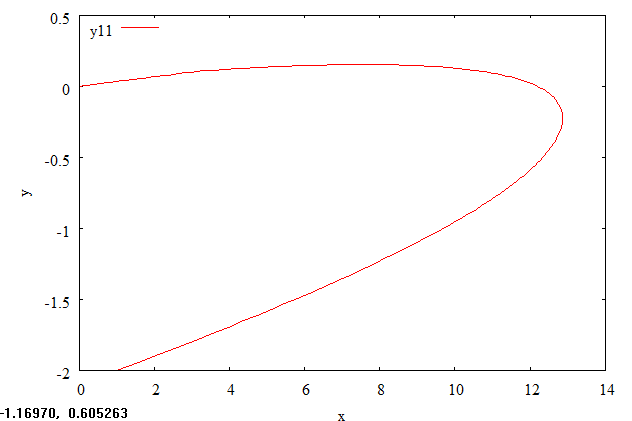
\includegraphics[width=0.7\textwidth]{task2_x}
\caption{Ãðàôèê $x(t)$}
\label{task2_x}
\end{figure}

\begin{figure}
\begin{floatrow}
\ffigbox{
    \caption{Ãðàôèê $u_1(t)$}
    \label{task2_u1}}
    {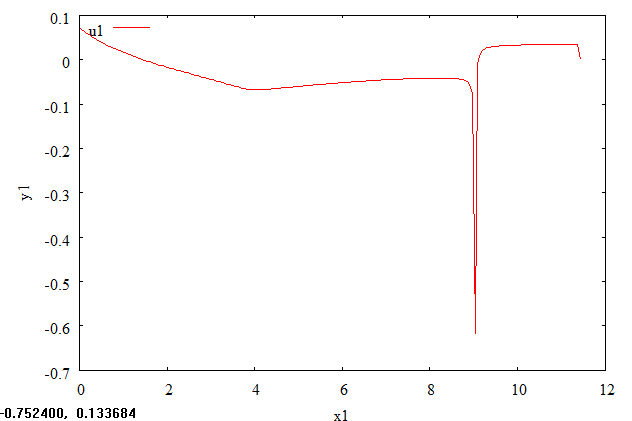
\includegraphics[width=0.5\textwidth]{task2_u1}}
\ffigbox{
    \caption{Ãðàôèê $u_2(t)$}
    \label{task2_u2}}
    {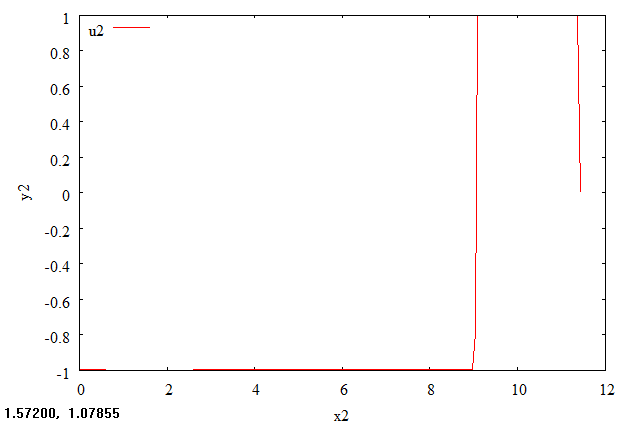
\includegraphics[width=0.5\textwidth]{task2_u2}}
\end{floatrow}
\end{figure}

\newpage
\section{Çàäà÷à áûñòðîäåéñòâèÿ ñ ïðîõîæäåíèåì çàäàííîé òî÷êè}
\subsection{Ïîñòàíîâêà çàäà÷è}

Ñèñòåìà èìååò âèä:

\begin{equation}\label{syst3}
\left\{ \begin{aligned}
& \ddot{x}+\alpha||\dot{x}||\dot{x} = \rho u, \; x,u \in \textbf{R}^2, \; \alpha,\rho > 0,\;  ||u|| \le 1, \\
& \ddot{y}+\beta||\dot{y}||\dot{y} = \sigma v, \; y,v \in \textbf{R}^2, \; \beta,\sigma > 0,\;  ||v|| \le 1, \\
& x(0)=x^0, \; \dot{x}(0) = \dot{x}^0, \; y(0)=y^0, \; \dot{y}(0) = \dot{y}^0, \\
& x(\tau)=x_t, \tau \in [0,T], \; x(T)=x_T, \\
& T \rightarrow \min_{||u|| \le 1},
\end{aligned}\right.
\end{equation}

Òàêæå äîëæíû âûïîëíÿòüñÿ íåðàâåíñòâà:

$$
    ||x(t)-y(t)|| \le 2, \; ||x(t)-y(t)|| \ge 1, \; t \in [0,T]. \\
$$


\subsection{Çàäà÷à íåëèíåéíîãî ïðîãðàììèðîâàíèÿ}

Çàäà÷à ÍËÏ çàïèñûâàåòñÿ ñ ïîìîùüþ ðàçíîñòíîé ñõåìû Ýéëåðà ñ ïåðåìåííûì øàãîì $$h = \begin{cases} \frac{\tau}{n_1}, & k=\overline{1,n_1} \\  \frac{T-\tau}{n_2}, & k=\overline{n_1,n_1+n_2} \end{cases} $$:

\begin{equation}\label{NLP3}
\left\{ \begin{aligned}
& x^1_{k} = x^1_{k-1} + h x^3_{k-1}, \\
& x^2_{k} = x^2_{k-1} + h x^4_{k-1}, \\
& x^3_{k} = x^3_{k-1} + h \Big(-\alpha \sqrt{(x^3_{k-1})^2+(x^4_{k-1})^2} x^3_{k-1} + \rho u^1_{k-1} \Big), \\
& x^4_{k} = x^4_{k-1} + h \Big(-\alpha \sqrt{(x^3_{k-1})^2+(x^4_{k-1})^2} x^4_{k-1} + \rho u^2_{k-1} \Big), \; k = \overline{1,n},
\end{aligned}\right.
\end{equation}

\begin{equation}\label{NLP32}
\left\{ \begin{aligned}
& y^1_{k} = y^1_{k-1} + h y^3_{k-1}, \\
& y^2_{k} = y^2_{k-1} + h y^4_{k-1}, \\
& y^3_{k} = y^3_{k-1} + h \Big(-\beta \sqrt{(y^3_{k-1})^2+(y^4_{k-1})^2} y^3_{k-1} + \sigma v^1_{k-1} \Big), \\
& y^4_{k} = y^4_{k-1} + h \Big(-\beta \sqrt{(y^3_{k-1})^2+(y^4_{k-1})^2} y^4_{k-1} + \sigma v^2_{k-1} \Big), \; k = \overline{1,n}.
\end{aligned}\right.
\end{equation}

Íà÷àëüíûå óñëîâèÿ îñòàþòñÿ òàêèìè æå, êàê â ïðåäûäóùåé çàäà÷å, ê êîòîððûì äîáàâëÿþòñÿ äâà óñëîâèÿ: $x_{n_1} = x_t, \; x_{n_1+n_2} = x_T$.

\subsection{Ðåøåíèå â GAMS}

Çàäà÷à ðåøàëàñü ïðè ñëåäóþùèõ çíà÷åíèÿõ ïàðàìåòðîâ:

$$
    x^1_0 = 0,\; x^2_0 = -5,\; x^3_0 = 1,\; x^4_0 = 2, \\
    y^1_0 = 0,\; y^2_0 = -6,\; x^3_0 = 1,\; x^4_0 = 0, \\
$$

$$
    x^1_t = 1,\; x^2_t = -2,\; x^1_T = 0,\; x^2_T = 0.
$$

À òàêæå $\rho = \sigma = 4,\; \alpha = \beta = 0.1$.

Îïòèìàëüíîå âðåìÿ $ T = 2.1 $. Íà Ðèñ. \ref{task3_xy},\ref{task3_u1},\ref{task3_u2},\ref{task3_v1} è \ref{task3_v2} èçîáðàæåíû ãðàôèêè òðàåêòîðèé è óïðàâëåíèé.

\begin{figure}
\centering
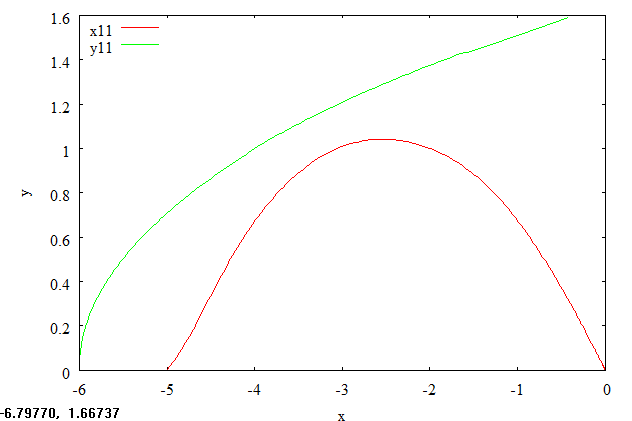
\includegraphics[width=0.7\textwidth]{task3_xy}
\caption{Ãðàôèê $x(t)$ è $y(t)$}
\label{task3_xy}
\end{figure}

\begin{figure}
\begin{floatrow}
\ffigbox{
    \caption{Ãðàôèê $u_1(t)$}
    \label{task3_u1}}
    {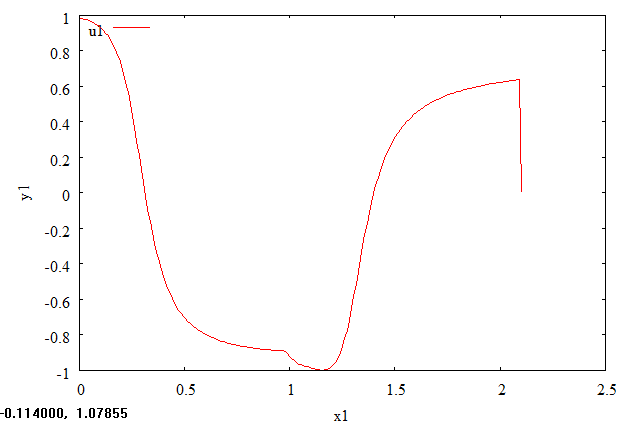
\includegraphics[width=0.5\textwidth]{task3_u1}}
\ffigbox{
    \caption{Ãðàôèê $u_2(t)$}
    \label{task3_u2}}
    {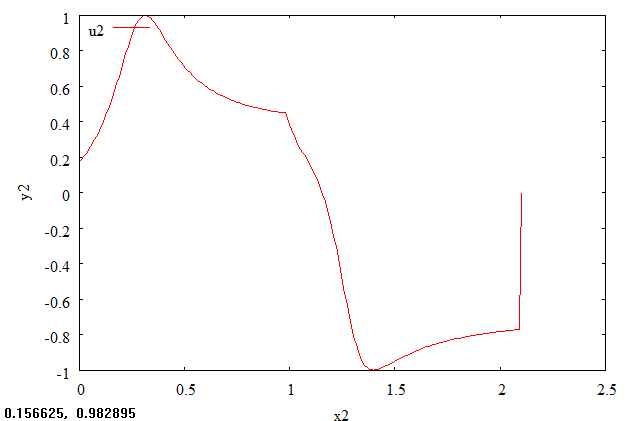
\includegraphics[width=0.5\textwidth]{task3_u2}}
\end{floatrow}
\end{figure}

\begin{figure}
\begin{floatrow}
\ffigbox{
    \caption{Ãðàôèê $v_1(t)$}
    \label{task3_v1}}
    {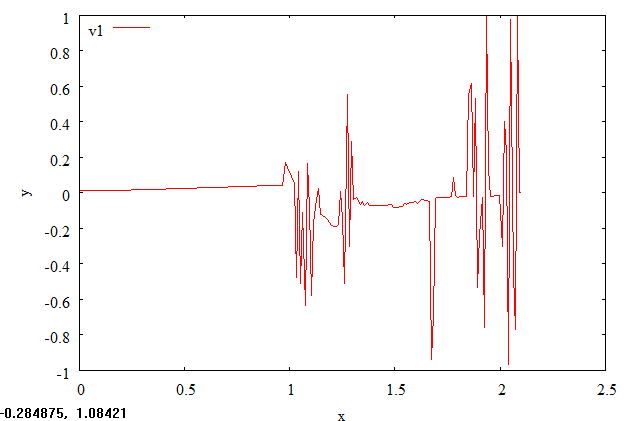
\includegraphics[width=0.5\textwidth]{task3_v1}}
\ffigbox{
    \caption{Ãðàôèê $v_2(t)$}
    \label{task3_v2}}
    {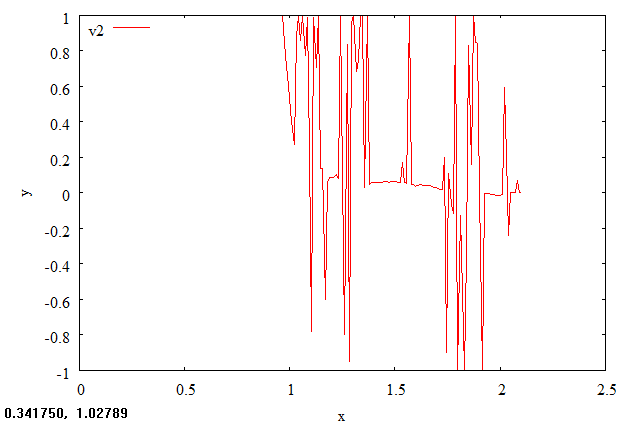
\includegraphics[width=0.5\textwidth]{task3_v2}}
\end{floatrow}
\end{figure}

\newpage
\section{Ðàçðàáîòêà êàðüåðà îòêðûòîãî òèïà}
\subsection{Ïîñòàíîâêà çàäà÷è}

Äèíàìèêà ðàçðàáîòêè êàðüåðà îïèñûâàåòñÿ ñëåäóþùèìè óðàâíåíèÿìè :

\begin{equation}\label{syst4}
\left\{ \begin{aligned}
& \dot{y} = f^0(u^1,P,Q), \;  y(0)=0, \; y(T) = y_T, \; 0 \le u_1 \le 1, \\
& \dot{P} = u^2, \; P(0) = P^0 \ge 0, \; 0 \le u_2 \le 1,\\
& \dot{Q} = u^2+u^3, \; Q(0) = Q^0 \ge 0, \; 0 \le u_3 \le 1, \\
& J = \int_0^T e^{-\nu t} \Big[ -m f^0 - u^2 - u^3 - p P + s(t)P(2-\frac{P}{f^0}) \Big] dt \rightarrow \max,
\end{aligned}\right.
\end{equation}
ãäå

$$
    f^0(u^1,P,Q) = u^1 P + (1 -u^1) Q.
$$

 äàííîé çàäà÷å $s(t)$ - áèðæåâûå öåíû íà ñûðü¸, äîñòóïíû èç ôàéëà $data.csv$, $p$ - öåíà ïåðåðàáîòêè åäèíèöû ñûðüÿ, $m$ - öåíà çà äîáû÷ó åäèíèöû ñûðüÿ. Âðåìÿ $T$ íå ôèêñèðîâàííî.

\subsection{Çàäà÷à íåëèíåéíîãî ïðîãðàììèðîâàíèÿ}

Ïðèâåäåì çàäà÷ó \eqref{syst4} ê çàäà÷å ÍËÏ:

\begin{equation}\label{NLP4}
\left\{ \begin{aligned}
& y_{k} = y_{k-1} + h f^0_{k-1}, \; y_0 = 0,\; y_n = y_T \\
& P_{k} = P_{k-1} + h u^2_{k-1}, \; P_0 = P^0, \\
& Q_{k} = Q_{k-1} + h (u^2_{k-1} + u^3_{k-1}), \; Q_0 = Q^0, \; k = \overline{1,n}. \\
\end{aligned}\right.
\end{equation}

Ôóíêöèîíàë çàïèøåòñÿ â ñëåäóþùåì âèäå:

$$
    J = \sum_{i=0}^n e^{-\nu ih}\Big( -m f^0_i - u^2_i - u^3_i -p P_i + s_i P_i (2-\frac{P_i}{f^0_i}) \Big).
$$


\subsection{Ðåøåíèå â GAMS}

Çàäà÷à ðåøàëàñü ïðè ñëåäóþùèõ çíà÷åíèÿõ ïàðàìåòðîâ:

$$
    m = 1,\;p=5,\;\nu=0.01,\;y_T=2000,\;P^0=0.8,\;Q^0=1.
$$

Ïîëó÷åííîå çíà÷åíèå ôóíêöèîíàëà $J = 6.7*10^6$. Ãðàôèêè òðàåêòîðèé è óïðàâëåíèÿ ïîêàçàíû íà Ðèñ.\ref{task4_P},\ref{task4_Q},\ref{task4_y},\ref{task4_u1},\ref{task4_u2} è \ref{task4_u3}.

\begin{figure}
\begin{floatrow}
\ffigbox{
    \caption{Ãðàôèê $P(t)$}
    \label{task4_P}}
    {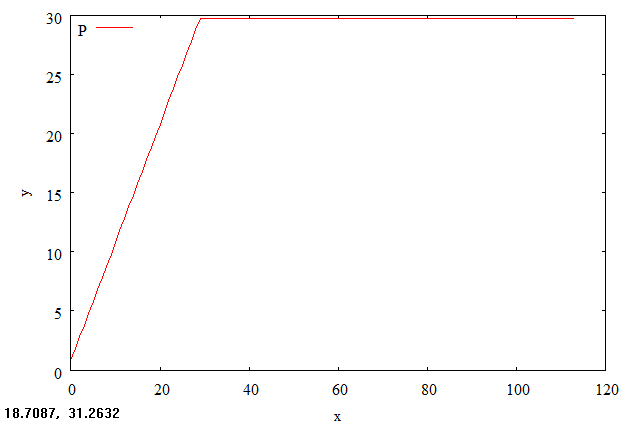
\includegraphics[width=0.5\textwidth]{task4_P}}
\ffigbox{
    \caption{Ãðàôèê $Q(t)$}
    \label{task4_Q}}
    {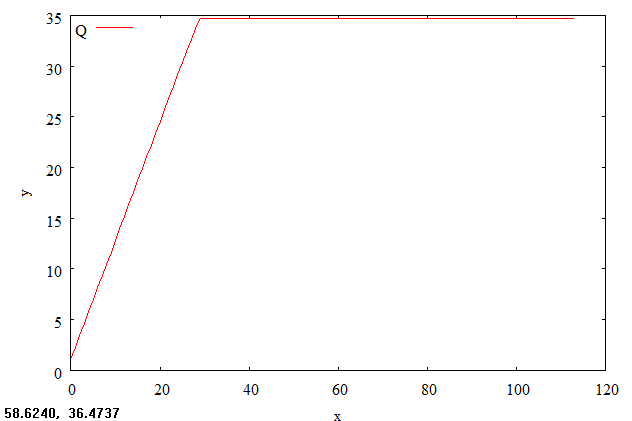
\includegraphics[width=0.5\textwidth]{task4_Q}}
\end{floatrow}
\end{figure}

\begin{figure}
\begin{floatrow}
\ffigbox{
    \caption{Ãðàôèê $y(t)$}
    \label{task4_y}}
    {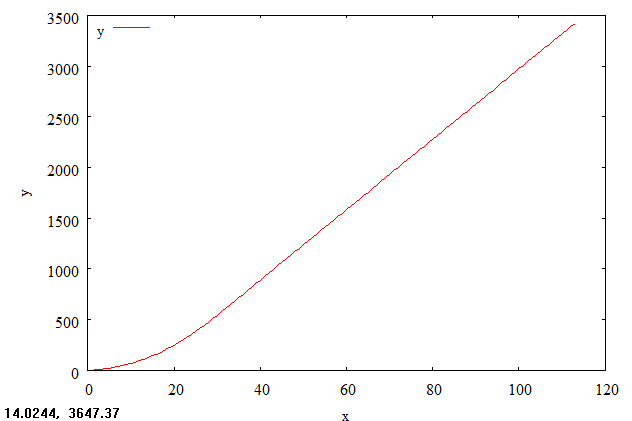
\includegraphics[width=0.5\textwidth]{task4_y}}
\ffigbox{
    \caption{Ãðàôèê $u_1(t)$}
    \label{task4_u1}}
    {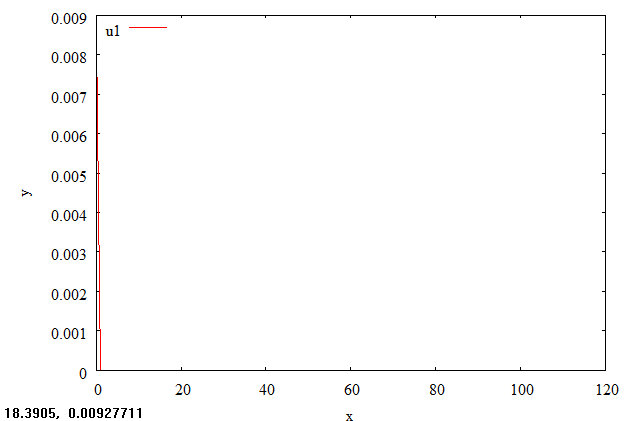
\includegraphics[width=0.5\textwidth]{task4_u1}}
\end{floatrow}
\end{figure}

\begin{figure}
\begin{floatrow}
\ffigbox{
    \caption{Ãðàôèê $u_2(t)$}
    \label{task4_u2}}
    {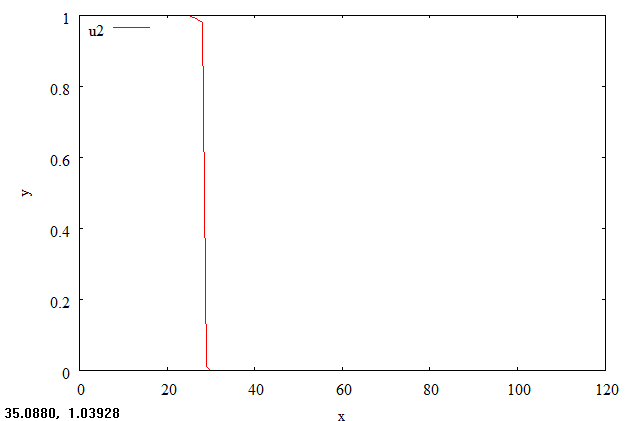
\includegraphics[width=0.5\textwidth]{task4_u2}}
\ffigbox{
    \caption{Ãðàôèê $u_3(t)$}
    \label{task4_u3}}
    {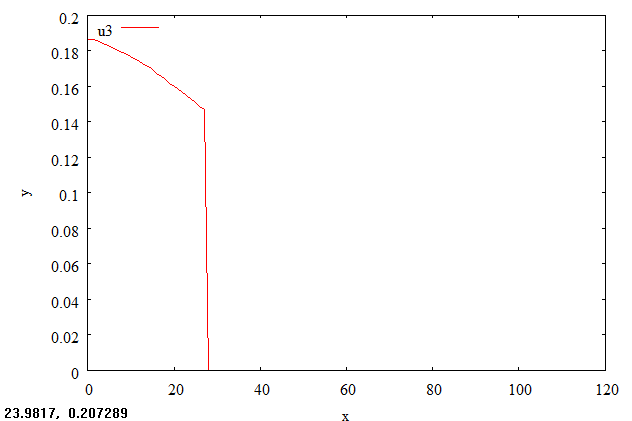
\includegraphics[width=0.5\textwidth]{task4_u3}}
\end{floatrow}
\end{figure}


\newpage
\section{Çàäà÷à ãðàíè÷íîãî Äèðèõëå óïðàâëåíèÿ äëÿ óðàâíåíèÿ êîëåáàíèé}
\subsection{Ïîñòàíîâêà çàäà÷è}

Óïðàâëÿåìûé ïðîöåññ $ y = y(t,x; u)$ :

\begin{equation}\label{syst5}
\left\{ \begin{aligned}
& y_{tt} = y_{xx}, \;  0 < t < T, \; 0 < x < l, \\
& y|_{x=0} = u(t), \; y|_{x=l} = 0, \;  0 < t < T, \\
& y|_{t=0} = 0, \; y_t|_{t=0} = 0, \;  0 < x < l, \\
& J(u) = \int_0^l \Big( |y_x(T,x;u) - \dot{f}^{0}(x)|^2 + |y_t(T,x;u) - f^1(x)|^2  \Big)  \rightarrow \inf,
\end{aligned}\right.
\end{equation}

Ïðåäïîëàãàåòñÿ âûïîëíåííûì óñëîâèå óïðàâëÿåìîñòè : $T > 2 l$.

\subsection{Çàäà÷à íåëèíåéíîãî ïðîãðàììèðîâàíèÿ}

Ïåðåõîäèì ê çàäà÷å íåëèíåéíîãî ïðîãðàììèðîâàíèÿ ñ ïîìîùüþ ïðîñòåéøåé ÿâíîé ñõåìû ñ øàáëîíîì <<êðåñò>> íà ðàâíîìåðíîé ñåòêå ñ øàãàìè $\tau = \frac{T}{m}$ ïî $t$ è $ h = \frac{l}{n}$ ïî $x$. Ïðè ýòîì äîëæíî âûïîëíÿòüñÿ óñëîâèå óñòîé÷èâîñòè: $\frac{\tau}{h} < 1$.

\begin{equation}\label{NLP2}
\left\{ \begin{aligned}
& \frac{y_i^{j+1}-2y_i^j+y_i^{j-1}}{\tau^2} = \frac{y_{i+1}^j-2y_i^j+y_{i-1}^j}{h^2}, \; i = \overline{1,n-1}, \; j = \overline{1,m-1}, \\
& y_0^j = u^j,\; y_n^j = 0,\;  j=\overline{1,m},\;  \\
& y_i^0 = 0 ,\; i = \overline{0,n},\; \frac{y_i^1 - y_i^0}{\tau} = 0,\; i = \overline{1,n-1},
\end{aligned}\right.
\end{equation}

Èíòåãðàë ñ÷èòàåì ìåòîäîì ïðÿìîóãîëüíèêîâ:

$$
    J = \sum_{i=1}^N\Big( \frac{y_i^m-y_{i-1}^m}{h} - \frac{f_i^0-f_{i-1}^0}{h}\Big)^2 h + \sum_{i=1}^{n-1} \Big(\frac{y_i^m-y_i^{m-1}}{\tau} - f_i^1\Big)^2 h \rightarrow \inf.
$$


\subsection{Ðåøåíèå â GAMS}

Çàäà÷à ðåøàëàñü ïðè ñëåäóþùèõ çíà÷åíèÿõ ïàðàìåòðîâ:$l = 1,\; T = 3 l = 3,$ è ôóíêöèÿõ $f^0(x) = xl-x^2,\; f^1(x) = \sin{\frac{\pi x}{l}}$.

Ïîëó÷åííîå çíà÷åíèå ôóíêöèîíàëà $J = 2.7*10^{-8}$. Ãðàôèêè óïðàâëåíèÿ è òðàåêòîðèé â êîíå÷íûé ìîìåíò âðåìåíè (â ñðàâíåíèè ñ æåëàåìûìè ôóíêöèÿìè $f^0(x)$ è $f^1(x)$) ïîêàçàíû íà Ðèñ.\ref{task5_u},\ref{task5_yT},\ref{task5_f0},\ref{task5_dyT} è \ref{task5_f1}.

\begin{figure}
\centering
\includegraphics[width=0.7\textwidth]{task5_u}
\caption{Ãðàôèê $u(t)$}
\label{task5_u}
\end{figure}

\begin{figure}
\begin{floatrow}
\ffigbox{
    \caption{Ãðàôèê $y(T,x)$}
    \label{task5_yT}}
    {\includegraphics[width=0.5\textwidth]{task5_yT}}
\ffigbox{
    \caption{Ãðàôèê $f^0(t)$}
    \label{task5_f0}}
    {\includegraphics[width=0.5\textwidth]{task5_f0}}
\end{floatrow}
\end{figure}

\begin{figure}
\begin{floatrow}
\ffigbox{
    \caption{Ãðàôèê $\dot{y}(T,x)$}
    \label{task5_dyT}}
    {\includegraphics[width=0.5\textwidth]{task5_dyT}}
\ffigbox{
    \caption{Ãðàôèê $f^1(t)$}
    \label{task5_f1}}
    {\includegraphics[width=0.5\textwidth]{task5_f1}}
\end{floatrow}
\end{figure}

\newpage
\section{Çàäà÷à î âñòðå÷å â èãðå äâóõ àâòîìîáèëåé}
\subsection{Ïîñòàíîâêà çàäà÷è}

Äâèæåíèå òî÷êè $X$ îïèñûâàåòñÿ ñèñòåìîé:

\begin{equation}\label{syst6}
\left\{ \begin{aligned}
& \dot{x_1} = x_3, \;  \dot{x_3} = \frac{x_4 u}{\sqrt{x_3^2+x_4^2}}, \\
& \dot{x_2} = x_4, \;  \dot{x_4} = - \frac{x_3 u}{\sqrt{x_3^2+x_4^2}}, \; ||u|| \le k.\\
\end{aligned}\right.
\end{equation}

Äâèæåíèå òî÷êè $Y$ îïèñûâàåòñÿ ñèñòåìîé:

\begin{equation}\label{syst7}
 \dot{y_1} = \omega_2\cos{y_3}, \;  \dot{y_2} = \omega_2\sin{y_3}, \; \dot{y_3} =  \frac{v}{\omega_2},\; ||v|| \le a,\\
\end{equation}
ãäå $\omega_2 = \sqrt{\dot{y}_1^2+\dot{y}_2^2}$ - ìîäóëü ñêîðîñòè $Y$.

Íà÷àëüíûå óñëîâèÿ èìåþò âèä:

$$
\begin{aligned}
& x_1(0) = x_2(0) = 0,\; y_1(0) = y_1^0,\; y_2(0) = y_2^0,\; y_3(0) = 0,\\
& x_3(0) = \frac{y_1^0 \omega_1}{\sqrt{(y_1^0)^2+(y_2^0)^2}}, \; x_4(0) = \frac{y_2^0 \omega_1}{\sqrt{(y_1^0)^2+(y_2^0)^2}}, \\
\end{aligned}
$$
ãäå $\omega_1 = \sqrt{\dot{x}_1^2+\dot{x}_2^2}$ - ìîäóëü ñêîðîñòè $X$.

Óñëîâèå îêîí÷àíèÿ èãðû èìååò âèä:

$$
    h(x_i(T),y_i(T)) = (x_1(T)-y_1(T))^2 + (x_2(T)-y_2(T))^2 - l^2 = 0.
$$

Öåëüþ îáúåêòà $X$ ÿâëÿåòñÿ äîñòèæåíèå âñòðå÷è çà êðàò÷àéøåå âðåìÿ $T$. Öåëü îáúåêòà $Y$ - èçáåæàòü âñòðå÷è, à åñëè ýòî íåâîçìîæíî, òî ìàêñèìèçèðîâàòü âðåìÿ $T$.

Çàäàäèì óïðàâëåíèå îáúåêòà $X$ ñîîòíîøåíèåì $u = k\sin{\phi}$, ãäå $\phi$ - óãîë ìåæäó âåêòîðîì ñêîðîñòè $X$ è íàïðàâëåíèåì $XY$.

Äâèæåíèå ðàññìàòðèâàåòñÿ íà êîíå÷íîì îòðåçêå âðåìåíè $[0,T_0]$.

\subsection{Çàäà÷à íåëèíåéíîãî ïðîãðàììèðîâàíèÿ}

Îáúåêò $X$:

\begin{equation}\label{NLP6}
\left\{ \begin{aligned}
& x^1_{k} = x^1_{k-1} + h x^3_{k-1}, \\
& x^2_{k} = x^2_{k-1} + h x^4_{k-1}, \\
& x^3_{k} = x^3_{k-1} + h \frac{x^4_{k-1} u_{k-1} }{\sqrt{(x^3_{k-1})^2+(x^4_{k-1})^2}} , \\
& x^4_{k} = x^4_{k-1} - h \frac{x^3_{k-1} u_{k-1} }{\sqrt{(x^3_{k-1})^2+(x^4_{k-1})^2}} , \; k = \overline{1,n}.
\end{aligned}\right.
\end{equation}


Îáúåêò $Y$:

\begin{equation}\label{NLP62}
\left\{ \begin{aligned}
& y^1_{k} = y^1_{k-1} + h \omega_2 \cos{y^3_{k-1}}, \\
& y^2_{k} = y^2_{k-1} + h \omega_2 \sin{y^3_{k-1}}, \\
& y^3_{k} = y^3_{k-1} + h \frac{v_{k-1}}{\omega_2} \; k = \overline{1,n},
\end{aligned}\right.
\end{equation}


\subsection{Ðåøåíèå â GAMS}

Çàäà÷à ðåøàëàñü ïðè ñëåäóþùèõ çíà÷åíèÿõ ïàðàìåòðîâ:
$$x^1_0 = x^2_0 = 0,\; y^1_0 = -2,\; y^2_0 = 10,\; y^3_0 =0,\; \omega_1 = 4.4,\; \omega_2 = 2,\;a=5,\;k=7,\; l=1,\; T_0 =20.$$
Áûëî ïîëó÷åíî, ÷òî âòîðîé èãðîê ìîæåò óêëîíèòüñÿ îò âñòðå÷è äî ìîìåíòà âðåìåíè $T_0$. Ãðàôèêè òðàåêòîðèé è óïðàâëåíèé ïîêàçàíû íà Ðèñ.\ref{task6_xy},\ref{task6_u} è \ref{task6_v}. À òàêæå ãðàôèê ðàññòîÿíèÿ ìåæäó îáúåêòàìè íà Ðèñ. \ref{task6_l}.

\begin{figure}
\begin{floatrow}
\ffigbox{
    \caption{Ãðàôèêè $x(t)$ è $y(t)$}
    \label{task6_xy}}
    {\includegraphics[width=0.5\textwidth]{task6_xy}}
\ffigbox{
    \caption{Ãðàôèê $l(t)$}
    \label{task6_l}}
    {\includegraphics[width=0.5\textwidth]{task6_l}}
\end{floatrow}
\end{figure}

\begin{figure}
\begin{floatrow}
\ffigbox{
    \caption{Ãðàôèê $u(t)$}
    \label{task6_u}}
    {\includegraphics[width=0.5\textwidth]{task6_u}}
\ffigbox{
    \caption{Ãðàôèê $v(t)$}
    \label{task6_v}}
    {\includegraphics[width=0.5\textwidth]{task6_v}}
\end{floatrow}
\end{figure}

\newpage
\section{Çàäà÷à Êîììèâîÿæåðà}
\subsection{Ïîñòàíîâêà çàäà÷è}

Èìååòñÿ $n$ ãîðîäîâ. Ðàññòîÿíèå ìåæäó ëþáîé ïàðîé ãîðîäîâ èçâåñòíû è ñîñòàâëÿþò $c_{ij}$. Êîììèâîÿæåð äîëæåí ïîñåòèòü âñå ãîðîäà, ïîáûâàâ â êàæäîì òîëüêî îäèí ðàç òàê, ÷òîáû ñóììàðíàÿ äëèíà ìàðøðóòà áûëà áû ìèíèìàëüíîé. Îïðåäåëèì ëîãè÷åñêèå ïåðåìåííûå çàäà÷è: $x_{ij} = 1$ , åñëè êîììèâîÿæåð ïåðååçæàåò èç ãîðîäà $i$ â ãîðîä $j$, è $x_{ij} = 0$, åñëè íå ïåðååçæàåò.

Òîãäà ìàòåìàòè÷åñêàÿ ìîäåëü âûãëÿäèò ñëåäóþùèì îáðàçîì:

\begin{equation}\label{syst8}
    F = \sum_{i=1}^n \sum_{j=1}^n c_{ij}x_{ij} \rightarrow \min_{x_{ij},u_i},
\end{equation}

ïðè îãðàíè÷åíèÿõ

$$
    \sum_{i=1}^n x_{ij} = 1, \; j = 1,..,n,
$$
- òîëüêî îäèí âúåçä â ãîðîä $j$,
$$
    \sum_{j=1}^n x_{ij} = 1, \; i = 1,..,n,
$$
- òîëüêî îäèí âúåçä â ãîðîä $i$, è ïðè óñëîâèå îòñóòñòâèÿ öèêëîâ:

$$
    u_i-u_j+(n-1)x_{ij} \le  n - 2, \; i \neq j, \; i,j = 2,..,n, \; u_i \ge 0.
$$


\subsection{Çàäà÷à íåëèíåéíîãî ïðîãðàììèðîâàíèÿ}

 äàííîé çàäà÷å çàäà÷à ÍËÏ è èñõîäíàÿ ïîñòàíîâêà ñîâïàäàþò.

\subsection{Ðåøåíèå â GAMS}

Ïðè ðåøåíèè èñïîëüçîâàëàñü ìàòðèöà $c(i,j)$, èçîáðàæåííàÿ íà Ðèñ.\ref{task7_c}.

\begin{figure}
\centering
\includegraphics[width=0.7\textwidth]{task7_c}
\caption{Òàáëèöà $c(i,j)$}
\label{task7_c}
\end{figure}

Ïîëó÷åííîå îïòèìàëüíîå çíà÷åíèå ôóíêöèîíàëà $F = 39$. Ñîîòâåòñòâóþùàÿ ìàòðèöà $x(i,j)$ ïðåäñòàâëåíà íà Ðèñ.\ref{task7_x}.

\begin{figure}
\centering
\includegraphics[width=0.7\textwidth]{task7_x}
\caption{Òàáëèöà $x(i,j)$}
\label{task7_x}
\end{figure}

\begin{thebibliography}{0}

\bibitem{Sam} À.~À.~Ñàìàðñêèé, ~À.~Â.~Ãóëèí.
\emph{×èñëåííûå ìåòîäû}. Íàóêà, 1989.

\bibitem{Davis} Ì.~Äæ.~Äýâèñ.
\emph{Äèôôåðåíöèàëüíàÿ ìîäåëü ñàõàðíîãî äèàáåòà}.
 êíèãå \emph{Ìàòåìàòè÷åñêîå ìîäåëèðîâàíèå}. Ðåäàêòîðû Äæ.~Ýíäðþñ, Ð.~Ìàê-~Ëîóí. Ìèð, 1979.

\bibitem{Cher} Ô.~Ë.~×åðíîóñüêî, ~À.~À.~Ìåëèêÿí.
\emph{Èãðîâûå çàäà÷è óïðàâëåíèÿ è ïîèñêà}. Íàóêà, 1978.

\bibitem{Aiz} Ð.~Àéçåêñ.
\emph{Äèôôåðåíöèàëüíûå èãðû}. Ìèð, 1967.

\bibitem{Sig} È.~Õ.~Ñèãàë, ~À.~Ï.~Èâàíîâà.
\emph{Ââåäåíèå â ïðèêëàäíîå äèñêðåòíîå ïðîãðàììèðîâàíèå}. Ôèçìàòëèò, 2007.


\end{thebibliography}

\end{document}